\documentclass[11pt]{article}

\usepackage[margin=1in]{geometry}
\usepackage{amsmath,amssymb,amsthm,tikz}
\usepackage{xsim}

\title{Real Numbers: Exercises}
\author{Antony Perez}
\date{\today}

\begin{document}

\maketitle

%==================================================
% Exercise 1
%==================================================

\begin{exercise}
Let $A,B,C,\ldots\subseteq X$. The complement of $A$ in $X$ is
\[
A^c=X\setminus A.
\]

\begin{description}
\item[(a)] Prove that $(A^c)^c=A$.

\item[(b)] Prove De Morgan's Laws:
\[
(A\cap B)^c=A^c\cup B^c,
\]
and deduce
\[
(A\cup B)^c=A^c\cap B^c.
\]

\item[(c)] Draw Venn diagrams illustrating these identities.

\item[(d)] Generalize these laws to arbitrary finite collections of sets.
\end{description}
\end{exercise}

\begin{solution}

\textbf{Part (a).}

$A^c$ is defined as $X\backslash A$. Let $x\in A^c$. This implies $x\notin A$. The complement of $A^c$ would be $(A^c)^c$, which would leave us with $x\notin (A^c)^c$, which is equivalent to $x\notin A$. Therefore, we have shown that $(A^c)^c=A$.

\bigskip

\textbf{Part (b).}

Let $x\in A\cap B$. The complement of this would be $X\backslash(A\cap B)$, which would leave us with $x\notin(A\cap B)^c$. This means that $x\notin A$ or $x\notin B$, which is equivalent to $x\in A^c$ or $x\in B^c$. Therefore, we have shown that
\[
(A\cap B)^c=A^c\cup B^c.
\]

\bigskip

\textbf{Part (c).}

\begin{center}
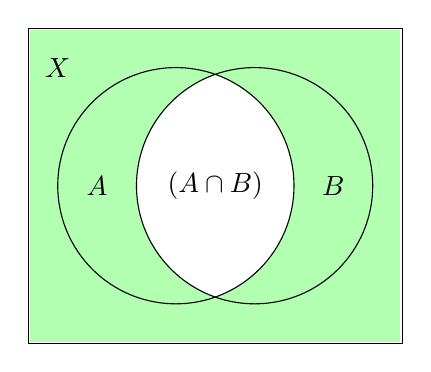
\begin{tikzpicture}

\draw (-.75,-1) rectangle (4,3);

\begin{scope}[shift={(1.125,1)}]

\fill[green!30] (-1.85,-1.98) rectangle (2.85,1.98);

\begin{scope}
\clip (0,0) circle (1.5cm);
\fill[white] (1,0) circle (1.5cm);
\end{scope}

\draw (0,0) circle (1.5cm);
\draw (1,0) circle (1.5cm);

\node at (-1,0) {$A$};
\node at (2,0) {$B$};
\node at (0.5,0) {$(A\cap B)$};
\node at (-1.5,1.5) {$X$};

\end{scope}

\end{tikzpicture}
\end{center}

\bigskip

\textbf{Part (d).}

Let's consider $n$ sets, and trying to generalize De Morgan's Laws. Let's assume these $n$ sets are $A_i\subset X$, where $i=1,2,\ldots,n$.

We can generalize De Morgan's Laws as follows:

\[
\bigcup_{i=1}^n A_i^c
=
\left(\bigcap_{i=1}^n A_i\right)^c
\Longleftrightarrow
\bigcap_{i=1}^n A_i^c
=
\left(\bigcup_{i=1}^n A_i\right)^c.
\]

\end{solution}

%==================================================
% Exercise 2
%==================================================

\begin{exercise}
\begin{description}
\item[(a)] Why does 4 divide every even integer square?
\item[(b)] Why does 8 divide every even integer cube?
\item[(c)] Why can 8 never divide twice an odd cube?
\item[(d)] Prove that the cube root of 2 is irrational.
\end{description}
\end{exercise}

\begin{solution}
\begin{proof}
    Part(a): An even integer can be represented as $2n$, where $n$ is an integer. Knowing this, we can square $2n$, and we arrive at $4n^2$, which is divisble by 4.
\end{proof}
\begin{proof}
    Part(b): An even integer can be represented as $2n$, where $n \in \mathbb{Z}$. Cubing $2n$, we arrive at $8n^3$, which is divisible by 8.  
\end{proof}
\begin{proof}
    Part(c): An odd integer can be represented as $2n+1$, where $n \in \mathbb{Z}$. Cubing $2n+1$, we arrive at $8n^3 + 12n^2 + 6n + 1$, which cannot be divided by 8 due to the remainder 1.
\end{proof}
\begin{proof}
    Part (d): Rational numbers are represented by $p/q, p,q \in \mathbb{Z}, q \neq 0$. Let's assume, for contradiction, that $\sqrt[3]{2}$ is rational, so $\sqrt[3]{2}=\frac{p}{q}$. Algebraic manipulation gives us $2q^3 = p^3$. Since the LHS is even, then the RHS must also be even, which implies that $p$ is even, since odd integers cubed only produce odd integers, and even integers cubed only produce even integers. Thus, we let $p = 2k$ for some integer $k$, and we arrive at $2q^3 = 8k^3 \rightarrow q^3 = 4k^3$. Now, since the RHS is even, the LHS must also be even, which implies that $q$ is even. This is a contradiction. Both $p$ and $q$ contain a factor of 2 which is divisible, thus showing that the rational expression was not in its simplest form. Therefore, $\sqrt[3]{2}$ is irrational.  
\end{proof}
\end{solution}

%==================================================
% Exercise 3
%==================================================

\begin{exercise}
Let $x=A\mid B$, $x'=A'\mid B'$ be cuts in $\mathbb{Q}$. We defined

\[
x+x'=(A+A')\mid\text{rest of }\mathbb{Q}.
\]

\begin{description}
    \item[(a)] Show that although $B+B'$ is disjoint from $A+A'$, it may happen in degenerate cases that $\mathbb{Q}$ is not the union of $A+A'$ and $B+B'$.
    \item[(b)] Infer that the definition of $x+x'$ as $(A+A') \mid (B+B')$ would be incorrect. 
    \item[(c)] Why did we not define $x \cdot x' = (A+A') \mid$ rest of $\mathbb{Q}$?  
\end{description}

\end{exercise}

\begin{solution}

\end{solution}

%=================================================
% Exercise 4
%=================================================

\begin{exercise}
Prove that there exists no smallest positive real number. Does there exist a smallest positive rational number? Given a real number $x$, does there exists a smallest real number $y > x$?
\end{exercise}

\begin{solution}

\end{solution}

%=================================================
% Exercise 5
%=================================================

\begin{exercise}
    Given $x>0$ and $n \in \mathbb{N}$, and $\epsilon > 0$, show that for some $\delta > 0$, if $u \in \mathbb{R}$ and $|u-y| < \delta$ then $|u^n-y^n| < \epsilon$ 
\end{exercise}

\begin{solution}

\end{solution}

%=================================================
% Exercise 6
%=================================================

\begin{exercise}
    Prove that real numbers correspond bijectively to decimal expansions not terminating in an infinite string of nines, as follows. The decimal expansion of $x \in \mathbb{R}$ is $N.x_1x_2\ldots$, where $N$ is the largest integer $\leq x,$ $x_1$ is the largest integer $\leq 10(x-N)$, $x_2$ is the largest integer $100(x-(N+x_1/10))$, and so on. 
    \begin{description}
        \item[(a)] Show that each $x_k$ is a digit between 0 and 9. 
        \item[(b)] Show that for each $k$ there is an $\ell \geq k$ such that $x_\ell \neq 9$.
        \item[(c)] Conversely, show that for each expansion $N.x_1x_2\ldots$ not terminating in an infinite stringe of nines, the set 
        \[
        \{N, N+ \frac{x_1}{10}, N+ \frac{x_1}{10} + \frac{x_2}{100}, \ldots\}
        \] 
        is bounded and its least upper bound is a real number $x$ with decimal expansion $N.x_1x_2\ldots$.
        \item[(d)] Repeat the exercise with a general base in place of 10. 
    \end{description}
\end{exercise}

\begin{solution}
    \begin{proof}
        Part(a): 
    \end{proof}
    \begin{proof}
        Part(b): 
    \end{proof}
\end{solution}

%=================================================
% Exercise 7
%=================================================

\begin{exercise}
    Let $f: A \rightarrow B$ be a function. That is, $f$ is some rule or device which when presented with any element $a \in A$, produces an element $b = f(a)$ of $B$. The graph of $f$ is the set $S$ of all pairs $(a,b) \in A \times B$ such that $b= f(a)$.

    \begin{description}
        \item[(a)] If you are given a subset $S \subset A \times B$, how can you tell if it is the graph of some function? (That is, what are the set theoretic properties of a graph?)
        \item[(b)] Let $g : B \rightarrow C$ be a second function and consider the composed function $g \circ f : A \rightarrow C$. Assume that $A=B=C=[0,1]$, draw $A \times B \times C$ as the unit cube in 3-space and try to relate the graphs of $f,g,$ and $g \circ f$ in the cube. 
    \end{description}

\end{exercise}

\begin{solution}
    
\end{solution}

%=================================================
% Exercise 8
%=================================================

\begin{exercise}
A rational number $p/q$ is dyadic if $q$ is a power of 2, $q=2^k$ for some nonnegative integer $k$. A dyadic interval is $[a,b]$ where $a = p^2k$ and $b=(p+1)/2^k$. A dyadic cube is the product of dyadic intervals having equal length. The set of dyadic rationals may be denoted as $\mathbb{Q}_2$ and the dyadic lattice as $\mathbb{Q}_2^m$.
\begin{description}
    \item[(a)] Prove that any two dyadic squares of the same size are either identical, intersect along a common edge, intersecct at a common vertex, or do not intersect at all. 
    \item[(b)] Show that the corresponding intersection property is true for dyadic cubes in $\mathbb{R}^m$.
\end{description}
\end{exercise}
\begin{solution}
    
\end{solution}

%================================================
% Exercise 9
%================================================

\begin{exercise}
    Given a cube in $\mathbb{R}^m$, what is the largest ball it contains? Given a ball in $\mathbb{R}^m$, what is the largest cube it contains? 
\end{exercise}
\begin{solution}
    
\end{solution}

%================================================
% Exercise 10
%================================================

\begin{exercise}
    Let $b(R)$ and $s(R)$ be the number of integer unit cubes in $\mathbb{R}^m$ that intersect the ball and sphere of radius $R$, centered at the origin.
    \begin{description}
        \item[(a)] Let $m=2$ and calculate the limits
        \[\lim_{R \rightarrow \infty} \frac{s(R)}{b(R)} \text{ and } \lim_{R \rightarrow \infty} \frac{s(R)^2}{b(R)}\]
        \item[(b)] Take $m \geq 3$. What exponent $k$ makes the limit interesting?  
        \[\lim_{R \rightarrow \infty} \frac{s(R)^k}{b(R)}\]
        \item[(c)] Let $c(R)$ be the number of integer unit cubes that are contained in the ball of radius $R$, cenetered at the origin. Calculate
        \[\lim_{R \rightarrow \infty} \frac{c(R)}{b(R)} \] 
        \item[(d)] Shift the ball to a new, arbitrary center and recalculate the limits.      
    \end{description}
\end{exercise}
\begin{solution}
    \begin{proof}
        $\lim_{R \rightarrow \infty} \frac{s(R)}{b(R)}=0, \lim_{R \rightarrow \infty} \frac{s(R)^2}{b(R)} = \frac{64}{\pi} $
    \end{proof}
\end{solution}

\printsolutions

\end{document}